\documentclass{beamer}

% \usepackage[orientation=landscape,size=custom,width=16,height=9,scale=0.6,debug]{beamerposter}

\usepackage{appendixnumberbeamer}
\usepackage{tikz}
\usetikzlibrary{arrows.meta}


\usetheme{Pittsburgh}
\setbeamertemplate{footline}[frame number]
\setbeamertemplate{navigation symbols}{}
\usecolortheme{beaver}
\setbeamertemplate{frametitle}[default][left]
\setbeamersize{text margin left=3em}
\usepackage{listings}
\usepackage{courier}

\def\glfdiagGF{black!10}
\def\glfdiagMMT{black!10}
\def\glfdiagShow#1{#1}
% \def\glfdiagHighlight{black!50!green!50}
\def\glfdiagHighlight{blue!70!green!60}

% \def\str#1{{\color{blue!70!green!80}``\textit{#1}''}}
\def\str#1{{\color{black!60!green}``\textit{#1}''}}

\newcommand{\com}[1]{\strut\hfil\strut\null\nobreak\hfill\hbox{{\itshape \color{black!50}#1}}\par}

\title{Prototyping Controlled Mathematical Languages in Jupyter Notebooks}

\author{\textbf{Jan Frederik Schaefer} \and Kai Amann \and Michael Kohlhase}
% \institute{\inst1Computer Science, FAU Erlangen-N\"urnberg \and \inst2Department of Computer Science and Engineering, Universit\`a di Bologna}
\institute{FAU Erlangen-N\"urnberg}
\date{\textbf{ICMS 2020} \\ remotely from Erlangen, Germany} % \\July 15/16, 2020}

\begin{document}

\begin{frame}
\titlepage
\end{frame}

\begin{frame}
    \frametitle{Introduction}
    \begin{itemize}
        \item Using math software requires learning input language
        \item Wouldn't it be nice to just use English?\com{really hard!}
        \item[$\rightarrow$] \textbf{Controlled mathematical languages}
            \com{= CNL for maths}
            \begin{itemize}
                \item Are formal languages for mathematics
                \item Have fixed semantics
                \item Imitate natural language
            \end{itemize}
    \end{itemize}

    \onslide<3->{
        \begin{itemize}
            \item Designing such languages is hard!
            \item Tool for prototyping: \textbf{GLF}\com{Grammatical Logical Framework}
            \item Contribution: Jupyter interface
        \end{itemize}
    }

    \vspace{1em}
    \only<1-3>{
        \centering
        \only<1>{
            \str{\lstinline[basicstyle=\ttfamily\upshape]{forall x \\ int(x) => even(x)}}
        }
        \only<2-3>{
            \str{Every integer is even.}
        }

        \vspace{0.3em}
        $\downarrow$

        \vspace{0.3em}
        $\forall x.\text{int}(x) \Rightarrow \text{even}(X)$
    }
    \only<4->{
        \centering
        \str{What is the cardinality of the alternating group on 5 symbols?}

        \vspace{0.3em}
        $\downarrow$

        \vspace{0.3em}
        \only<4>{compute(cardinality(alternating\_group(int\_term(5))))}
        \only<5>{
            \lstinline[language=Python,keepspaces=true,columns=fixed,basicstyle=\ttfamily]|print(AlternatingGroup(5).cardinality())|
        }
    }

\end{frame}

% \begin{frame}
%     \frametitle{Grammatical Logical Framework (GLF)}
% 
%     \begin{itemize}
%         \item Approach in natural-language semantics: \small\com{Montague 1970}
%         {
%             \vspace{0.5em}
%             \begin{tikzpicture}[xscale=1.05,yscale=0.9]
%                 \tikzset{ll/.style={line width=0.7pt}}
%                 \node[ll,fill=white,draw,minimum width=2cm,minimum height=1cm] (utt) at (-3.5,1.8) {String};
%                 \draw[ll,fill=white] (-1,1) -- (0,3) -- (1,1) -- cycle;
%                 \node[] (st) at (0,1.5) {AST};
%                 \draw[ll,-{Straight Barb[length=6.3,width=5.0]}] (-2.5, 1.8) to[bend left=15] node[above] {\footnotesize parsing} (-0.8,1.8);
%                 \draw[thick,fill=white] (2.5,1) -- (3.5,3) -- (4.5,1) -- cycle;
%                 \node (qlf) at (3.5,1.5) {\begin{tabular}{c}Logic\\Expression\end{tabular}};
%                 \draw[thick,-{Straight Barb[length=6.3,width=5.0]}] (0.8,1.8) to[bend left=15] node[above] {\footnotesize semantics} node[below]{\footnotesize construction} (2.7,1.8);
%             \end{tikzpicture}
%             \vspace{0.5em}
%         }
%         \item We have a tool for this: \textbf{GLF} \small \com{Grammatical Logical Framework}
%         \item User interface through Jupyter
%         \item Design controlled mathematical languages with GLF
%     \end{itemize}
% \end{frame}

\begin{frame}[fragile]
    \frametitle{Grammatical Logical Framework (GLF)}

        Combine two existing frameworks:
        \begin{itemize}
            \item \textbf{GF} (\emph{Grammatical Framework}) for grammar development
            \item \textbf{MMT} for logic development/semantics construction
        \end{itemize}

    \vspace{1em}
        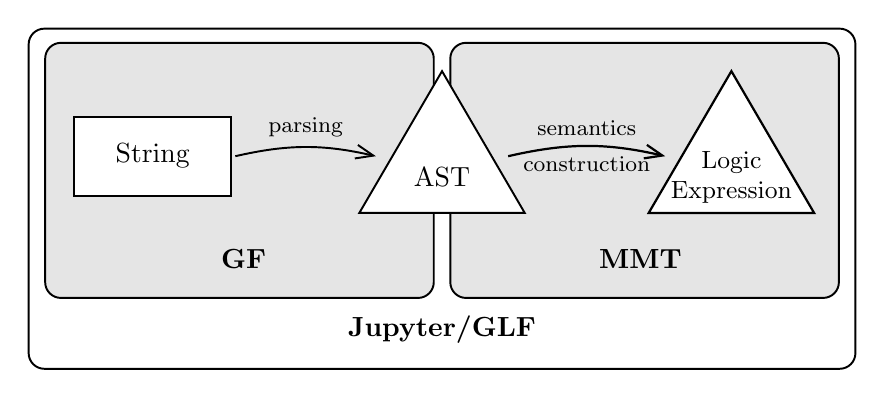
\begin{tikzpicture}[xscale=1.05,yscale=0.9]
    \tikzset{ll/.style={line width=0.7pt}}
    \draw[rounded corners=.2cm,color=white,fill=white] (-5.0,3.6) rectangle (5.0,-1.2);
    \glfdiagShow{
        \draw[ll,rounded corners=.2cm,fill=\glfdiagGF] (-4.8,3.4) rectangle (-0.1,-0.2);
        \draw[ll,rounded corners=.2cm,fill=\glfdiagMMT] (0.1,3.4) rectangle (4.8,-0.2);
        \draw[ll,rounded corners=.2cm] (-5.0,3.6) rectangle (5.0,-1.2);
        \node (gf) at (-2.4,0.35) {\textbf{GF}};
        \node (mmt) at (2.4,0.35) {\textbf{MMT}};
        \node (glf) at (0,-0.65) {\textbf{Jupyter/GLF}};
    }

    % rectangle and triangles have same area
    \node[ll,fill=white,draw,minimum width=2cm,minimum height=1cm] (utt) at (-3.5,1.8) {String};
    \draw[ll,fill=white] (-1,1) -- (0,3) -- (1,1) -- cycle;
    % \node[] (st) at (0,1.5) {\begin{tabular}{c}Parse\\Tree\end{tabular}};
    \node[] (st) at (0,1.5) {AST};
    \draw[ll,-{Straight Barb[length=6.3,width=5.0]}] (-2.5, 1.8) to[bend left=15] node[above] {\footnotesize parsing} (-0.8,1.8);
    \draw[thick,fill=white] (2.5,1) -- (3.5,3) -- (4.5,1) -- cycle;
    \node (qlf) at (3.5,1.5) {\small\begin{tabular}{c}Logic\\Expression\end{tabular}};
    \draw[thick,-{Straight Barb[length=6.3,width=5.0]}] (0.8,1.8) to[bend left=15] node[above] {\footnotesize semantics} node[below]{\footnotesize construction} (2.7,1.8);
\end{tikzpicture}

\end{frame}

\begin{frame}
    \frametitle{GF in Jupyter: Grammar Development}
%     \only<2>{
%         \begin{minipage}{0.6\textwidth}
%             \begin{block}{Core Functionality}
%                 \begin{itemize}
%                     \item Start GF shell in background
%                     \item Code cells contain:
%                         \begin{itemize}
%                             \item GF grammar modules
%                             \item GF commands
%                         \end{itemize}
%                     \item Save and import grammar modules
%                     \item Execute shell commands
%                 \end{itemize}
%             \end{block}
%         \end{minipage}
%     }
    \only<1>{
        \centering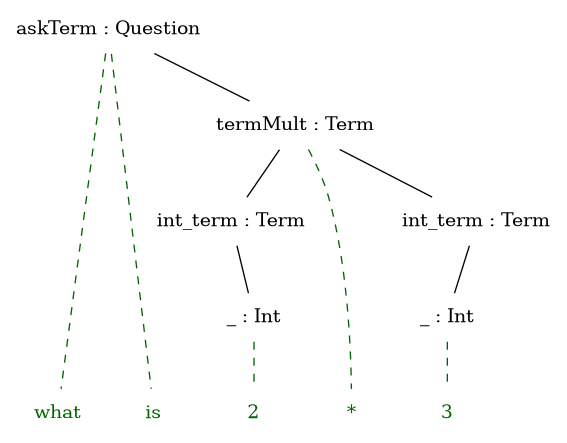
\includegraphics[scale=0.4]{ast.png}
    }
% 
%     \only<2>{
%     \vspace{1em}
%         \begin{block}{Further Features}
%             \begin{itemize}
%                 \item Generating stubs via tab-completion
%                 \item Extend GF commands with kernel commands
%                 \item Displaying trees in widgets
%             \end{itemize}
%         \end{block}
%     }
\end{frame}

\begin{frame}
    \frametitle{Grammatical Logical Framework (GLF)}
    % \begin{minipage}{0.3\textwidth}\centering\small\str{Every integer is even.}\end{minipage} $\;\mapsto\;$ 
\resizebox{0.2\textwidth}{!}{
    \begin{tikzpicture}[baseline=0.0em]
        \node[line width=0,rounded corners=.2cm,fill=gray!25] (abs) at (0,0) {
            \begin{tikzpicture}
                \node (a) at (-1, 0) {every};
                \node (j) at (-1, -.8) {integer};
                \node (h) at (1, 0) {even};
                \node (s) at (0, .8) {simpleStmt};
                \draw (a) -- (s);
                \draw (h) -- (s);
                \draw (a) -- (j);
            \end{tikzpicture}
        };
    \end{tikzpicture}
} $\;\mapsto\;$
\begin{minipage}{0.29\textwidth}
    \centering
    \footnotesize
    $\forall x.\text{int}(x) \Rightarrow \text{even}(X)$
\end{minipage}


    \vspace{1em}
        \def\glfdiagMMT{\glfdiagHighlight}
        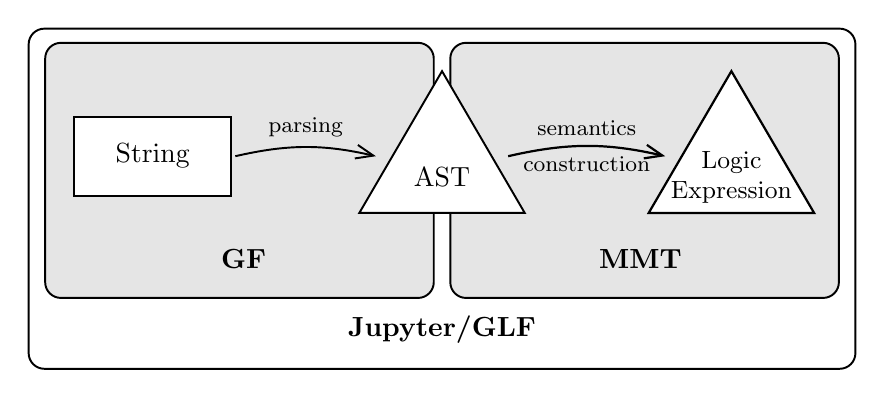
\begin{tikzpicture}[xscale=1.05,yscale=0.9]
    \tikzset{ll/.style={line width=0.7pt}}
    \draw[rounded corners=.2cm,color=white,fill=white] (-5.0,3.6) rectangle (5.0,-1.2);
    \glfdiagShow{
        \draw[ll,rounded corners=.2cm,fill=\glfdiagGF] (-4.8,3.4) rectangle (-0.1,-0.2);
        \draw[ll,rounded corners=.2cm,fill=\glfdiagMMT] (0.1,3.4) rectangle (4.8,-0.2);
        \draw[ll,rounded corners=.2cm] (-5.0,3.6) rectangle (5.0,-1.2);
        \node (gf) at (-2.4,0.35) {\textbf{GF}};
        \node (mmt) at (2.4,0.35) {\textbf{MMT}};
        \node (glf) at (0,-0.65) {\textbf{Jupyter/GLF}};
    }

    % rectangle and triangles have same area
    \node[ll,fill=white,draw,minimum width=2cm,minimum height=1cm] (utt) at (-3.5,1.8) {String};
    \draw[ll,fill=white] (-1,1) -- (0,3) -- (1,1) -- cycle;
    % \node[] (st) at (0,1.5) {\begin{tabular}{c}Parse\\Tree\end{tabular}};
    \node[] (st) at (0,1.5) {AST};
    \draw[ll,-{Straight Barb[length=6.3,width=5.0]}] (-2.5, 1.8) to[bend left=15] node[above] {\footnotesize parsing} (-0.8,1.8);
    \draw[thick,fill=white] (2.5,1) -- (3.5,3) -- (4.5,1) -- cycle;
    \node (qlf) at (3.5,1.5) {\small\begin{tabular}{c}Logic\\Expression\end{tabular}};
    \draw[thick,-{Straight Barb[length=6.3,width=5.0]}] (0.8,1.8) to[bend left=15] node[above] {\footnotesize semantics} node[below]{\footnotesize construction} (2.7,1.8);
\end{tikzpicture}

\end{frame}


% \begin{frame}
%     \frametitle{MMT in Jupyter: Logic Development}
%     \begin{block}{Core Functionality}
%         \begin{itemize}
%             \item Start MMT as server
%             \item Recognize MMT content and import it
%             \item Automatically import abstract syntaxes
%             \item Add command for semantics construction
%         \end{itemize}
%     \end{block}
% 
%     \begin{block}{Further Features}
%         \begin{itemize}
%             \item Stub generation via tab-completion
%             \item Unicode characters via tab-completion
%         \end{itemize}
%     \end{block}
% \end{frame}

\begin{frame}
    \frametitle{Jupyter/GLF}
    % \begin{minipage}{0.3\textwidth}\centering\small\str{Every integer is even.}\end{minipage} $\;\mapsto\;$ 
\resizebox{0.2\textwidth}{!}{
    \begin{tikzpicture}[baseline=0.0em]
        \node[line width=0,rounded corners=.2cm,fill=gray!25] (abs) at (0,0) {
            \begin{tikzpicture}
                \node (a) at (-1, 0) {every};
                \node (j) at (-1, -.8) {integer};
                \node (h) at (1, 0) {even};
                \node (s) at (0, .8) {simpleStmt};
                \draw (a) -- (s);
                \draw (h) -- (s);
                \draw (a) -- (j);
            \end{tikzpicture}
        };
    \end{tikzpicture}
} $\;\mapsto\;$
\begin{minipage}{0.29\textwidth}
    \centering
    \footnotesize
    $\forall x.\text{int}(x) \Rightarrow \text{even}(X)$
\end{minipage}

    \begin{itemize}
        \item Run GF and MMT in background
        \item Identify content using pattern matching
        \item Tab completion for stub generation
    \end{itemize}

    \vspace{1em}
    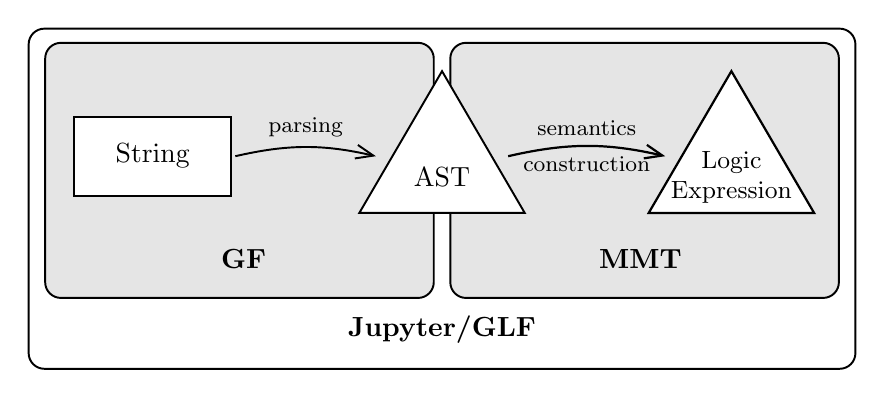
\begin{tikzpicture}[xscale=1.05,yscale=0.9]
    \tikzset{ll/.style={line width=0.7pt}}
    \draw[rounded corners=.2cm,color=white,fill=white] (-5.0,3.6) rectangle (5.0,-1.2);
    \glfdiagShow{
        \draw[ll,rounded corners=.2cm,fill=\glfdiagGF] (-4.8,3.4) rectangle (-0.1,-0.2);
        \draw[ll,rounded corners=.2cm,fill=\glfdiagMMT] (0.1,3.4) rectangle (4.8,-0.2);
        \draw[ll,rounded corners=.2cm] (-5.0,3.6) rectangle (5.0,-1.2);
        \node (gf) at (-2.4,0.35) {\textbf{GF}};
        \node (mmt) at (2.4,0.35) {\textbf{MMT}};
        \node (glf) at (0,-0.65) {\textbf{Jupyter/GLF}};
    }

    % rectangle and triangles have same area
    \node[ll,fill=white,draw,minimum width=2cm,minimum height=1cm] (utt) at (-3.5,1.8) {String};
    \draw[ll,fill=white] (-1,1) -- (0,3) -- (1,1) -- cycle;
    % \node[] (st) at (0,1.5) {\begin{tabular}{c}Parse\\Tree\end{tabular}};
    \node[] (st) at (0,1.5) {AST};
    \draw[ll,-{Straight Barb[length=6.3,width=5.0]}] (-2.5, 1.8) to[bend left=15] node[above] {\footnotesize parsing} (-0.8,1.8);
    \draw[thick,fill=white] (2.5,1) -- (3.5,3) -- (4.5,1) -- cycle;
    \node (qlf) at (3.5,1.5) {\small\begin{tabular}{c}Logic\\Expression\end{tabular}};
    \draw[thick,-{Straight Barb[length=6.3,width=5.0]}] (0.8,1.8) to[bend left=15] node[above] {\footnotesize semantics} node[below]{\footnotesize construction} (2.7,1.8);
\end{tikzpicture}

\end{frame}


\begin{frame}
    \frametitle{Jupyter/GLF for Larger Projects}
    \begin{itemize}
        \item Implement grammar/logic/semantics construction externally
        \item Use Jupyter notebooks for
            \begin{itemize}
                \item Experimenting with specific challenges
                \item Testing
                \item Demos
            \end{itemize}
        \item Case study: GLForTheL \com{re-implement ForTheL in GLF}
    \end{itemize}

    \vspace{2em}
    \centering
    \str{a subset of S is a set T such that every element of T belongs to S}
    
    \vspace{0.2em}
    $\downarrow$

    \vspace{0.2em}
    $\forall T. T \subseteq S \quad \Leftrightarrow\quad set(T) \wedge \forall x.x\in T \Rightarrow belongto(x,S)$
%     \footnotesize $\forall T.(subsetof\;T\;S)\Leftrightarrow(set\;T)\wedge\forall
%        x.(elementof\;x\;T)\wedge\top\Rightarrow(belongto\;x\;S)\wedge\top.$
\end{frame}

\begin{frame}
    \frametitle{Jupyter/GLF For Teaching}
    \begin{itemize}
        \item Used in 1-semester course on logic-based language processing
        \item Homework assignments:
            \begin{itemize}
                \item Provide partial implementations + explanations
                \item Easier to set up
                \item Was preferred by most students
            \end{itemize}
        \item Presentation in Classroom
            \begin{itemize}
                \item Interactive development with students
                \item Easy to share after lecture
            \end{itemize}
    \end{itemize}

    \centering
    \vspace{1em}
    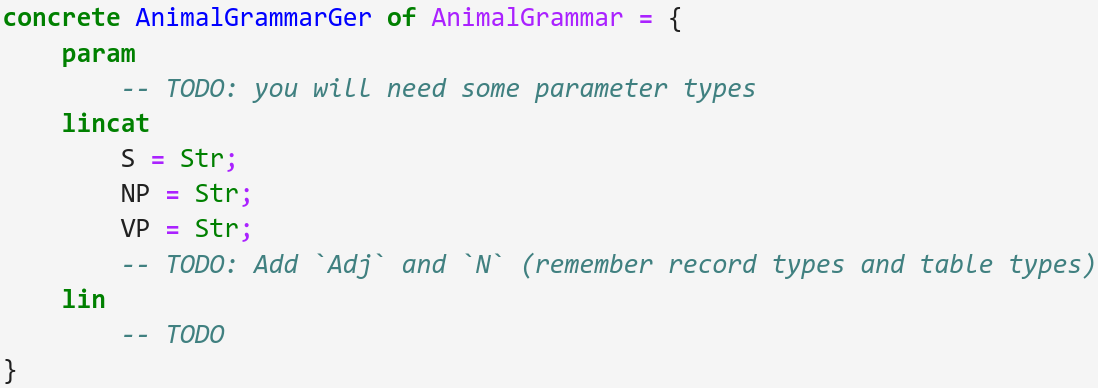
\includegraphics[scale=0.22]{problem.png}
\end{frame}

\begin{frame}
    \frametitle{Recent Development: GLIF}
    \begin{itemize}
        \item We need inference \com{e.g. for ambiguity resolution}
        \item We added ELPI (an extension of $\lambda$Prolog) to the pipeline
        \item Signatures can be generated from MMT
        \item First experiments with prover generation
    \end{itemize}

    \centering
    \vspace{2em}
    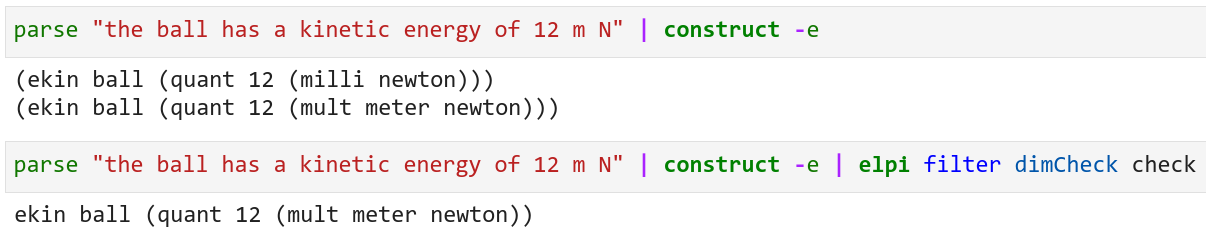
\includegraphics[scale=0.3]{filter.png}
%     \vspace{1.5em}
%     Example:
%     \begin{itemize}
%         \item \str{$12 mN$} could mean 
%             \begin{itemize}
%                 \item \str{12 meter Newton}
%                 \item \str{12 milli Newton}
%             \end{itemize}
%         \item In \str{an energy of $12 mN$} we can discard one reading
%         \item[$\rightarrow$] Use ELPI for dimensional analysis
%     \end{itemize}
\end{frame}

\begin{frame}
    \frametitle{Summary}
    \begin{itemize}
        \item We presented a Jupyter kernel for GLF \com{now GLIF}
        \item Kernel distinguishes content types with pattern matching:
            \begin{itemize}
                \item GF grammar modules
                \item MMT content
                \item Commands \com{handled by kernel/passed to GF}
            \end{itemize}
        \item Used for: teaching, prototyping, sharing results/demos, \dots
    \end{itemize}

    \vspace{0.8em}
    \centering
    \resizebox{0.6\textwidth}{!}{
        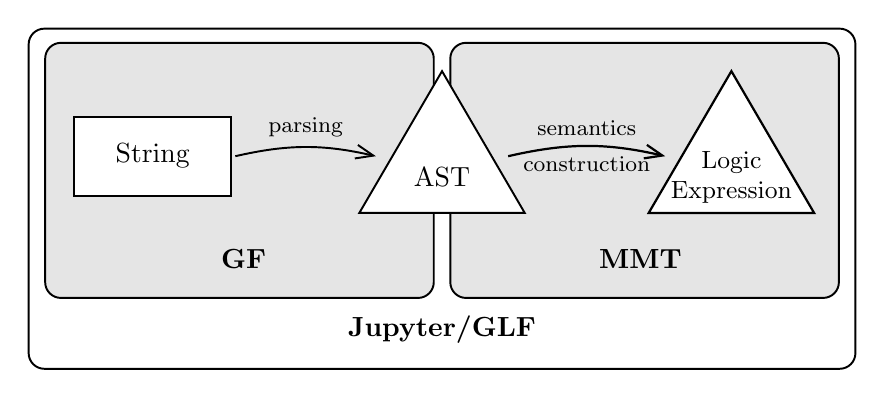
\begin{tikzpicture}[xscale=1.05,yscale=0.9]
    \tikzset{ll/.style={line width=0.7pt}}
    \draw[rounded corners=.2cm,color=white,fill=white] (-5.0,3.6) rectangle (5.0,-1.2);
    \glfdiagShow{
        \draw[ll,rounded corners=.2cm,fill=\glfdiagGF] (-4.8,3.4) rectangle (-0.1,-0.2);
        \draw[ll,rounded corners=.2cm,fill=\glfdiagMMT] (0.1,3.4) rectangle (4.8,-0.2);
        \draw[ll,rounded corners=.2cm] (-5.0,3.6) rectangle (5.0,-1.2);
        \node (gf) at (-2.4,0.35) {\textbf{GF}};
        \node (mmt) at (2.4,0.35) {\textbf{MMT}};
        \node (glf) at (0,-0.65) {\textbf{Jupyter/GLF}};
    }

    % rectangle and triangles have same area
    \node[ll,fill=white,draw,minimum width=2cm,minimum height=1cm] (utt) at (-3.5,1.8) {String};
    \draw[ll,fill=white] (-1,1) -- (0,3) -- (1,1) -- cycle;
    % \node[] (st) at (0,1.5) {\begin{tabular}{c}Parse\\Tree\end{tabular}};
    \node[] (st) at (0,1.5) {AST};
    \draw[ll,-{Straight Barb[length=6.3,width=5.0]}] (-2.5, 1.8) to[bend left=15] node[above] {\footnotesize parsing} (-0.8,1.8);
    \draw[thick,fill=white] (2.5,1) -- (3.5,3) -- (4.5,1) -- cycle;
    \node (qlf) at (3.5,1.5) {\small\begin{tabular}{c}Logic\\Expression\end{tabular}};
    \draw[thick,-{Straight Barb[length=6.3,width=5.0]}] (0.8,1.8) to[bend left=15] node[above] {\footnotesize semantics} node[below]{\footnotesize construction} (2.7,1.8);
\end{tikzpicture}

    }

    \vspace{0.8em}
    \large \url{https://github.com/KWARC/GLIF}
\end{frame}

\end{document}
